\chapter{Modelo del sistema solvatado}\label{chapter:apendicea}

\textcolor{red}{Encabezados de tablas}

% \section{Parámetros de los modelos}

% \subsection{Modelo de agua}

% El modelo de agua elegido para estas simulaciones fue el modelo SPC/E(punto simple punto de carga extendido) rígido, tiene cargas situadas en los tres átomos y la interacción Lennard-Jones con otras moléculas esta situada en el oxígeno. La figura (\ref{fig:SPCE}) es una visualización de la molécula y la tabla (\ref{SPCEpar}) son los parámetros del modelo.

% \begin{figure}[!h]
%     \centering
%     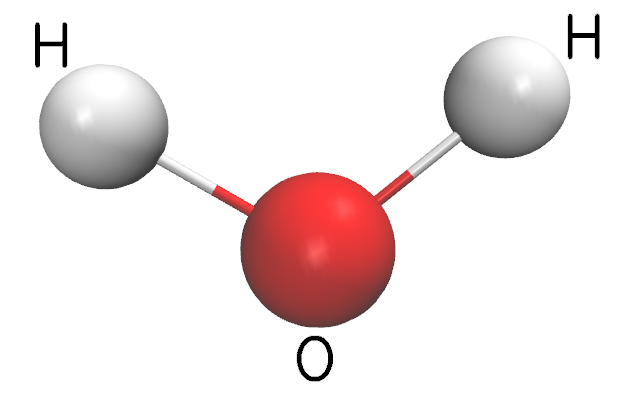
\includegraphics[width=.9\textwidth,keepaspectratio=true]{SPCE.png}
%     \caption{Molécula de agua}
%     \label{fig:SPCE}
% \end{figure}

% \begin{table}[h!]
%     \centering

%     \begin{tabular}{ |p{1cm}|p{4cm}|  }
%     \hline
%     $\sigma$  & 3.166 \AA \\
%     $\epsilon$& 0.650 KJ $mol^{-1}$ \\
%     $r_{OH}$  & 1.000 \AA \\
%     $\angle_{HOH}$&109.47 deg \\
%     $q_{O}$   & -0.8476 e \\
%     $q_{H}$   & 0.4238 e \\
%     \hline
%     \end{tabular}
%     \caption{Parámetros del modelo SPCE}
%     \label{SPCEpar}
% \end{table}

% \newpage

El sistema se compone de un nanotubo de carbono (6,5) y 10 moléculas de 2,4D. La siguientes tablas contienen los parámetros de simulación.

\begin{table}[!h]
    \centering
    \begin{tabular}{|l|c|l|c|}
    \hline
    Parámetro & valor & Parámeto & valor \\
    \hline
    $\epsilon_{cc}$ & 0.4058kJ/mol & $q_{o}$   & -0.8476e \\
    $\epsilon_{oo}$ & 0.6502kJ/mol &  $q_H$    & 0.4238e \\
    $\epsilon_{co}$ & 0.5137kJ/mol & $K^b_{CC}$& 3.2236X$10^6$ $\frac{kJ}{molnm^4}$\\
    $\sigma_{cc}$   & 3.361        & $b_{ij}$  & 1.42 \AA\\
    $\sigma_{oo}$   & 3.166        & $K^{\theta}_{CCC}$& 560 $\frac{kJ}{mol}$ \\
    $\sigma_{co}$   & 3.262        & $\theta^0_{ijk}$  & $120^{\circ}$ \\
    $r_{OH}$        & 1 \AA        & $k^{\phi}_{CCCC}$ & 5.86 $\frac{kJ}{mol}$ \\
    $\theta_{HOH}$  & $109.47^{\circ}$ & $\phi_s$         & $180^{\circ}$ \\
    \hline
    \end{tabular}
    \caption{Parámetros del modelo SPCE de agua y del nanotubo de carbono. \cite{meng2008}}
    \label{tab:cnth2oparameters}
\end{table}

\begin{figure}[!h]
    \centering
    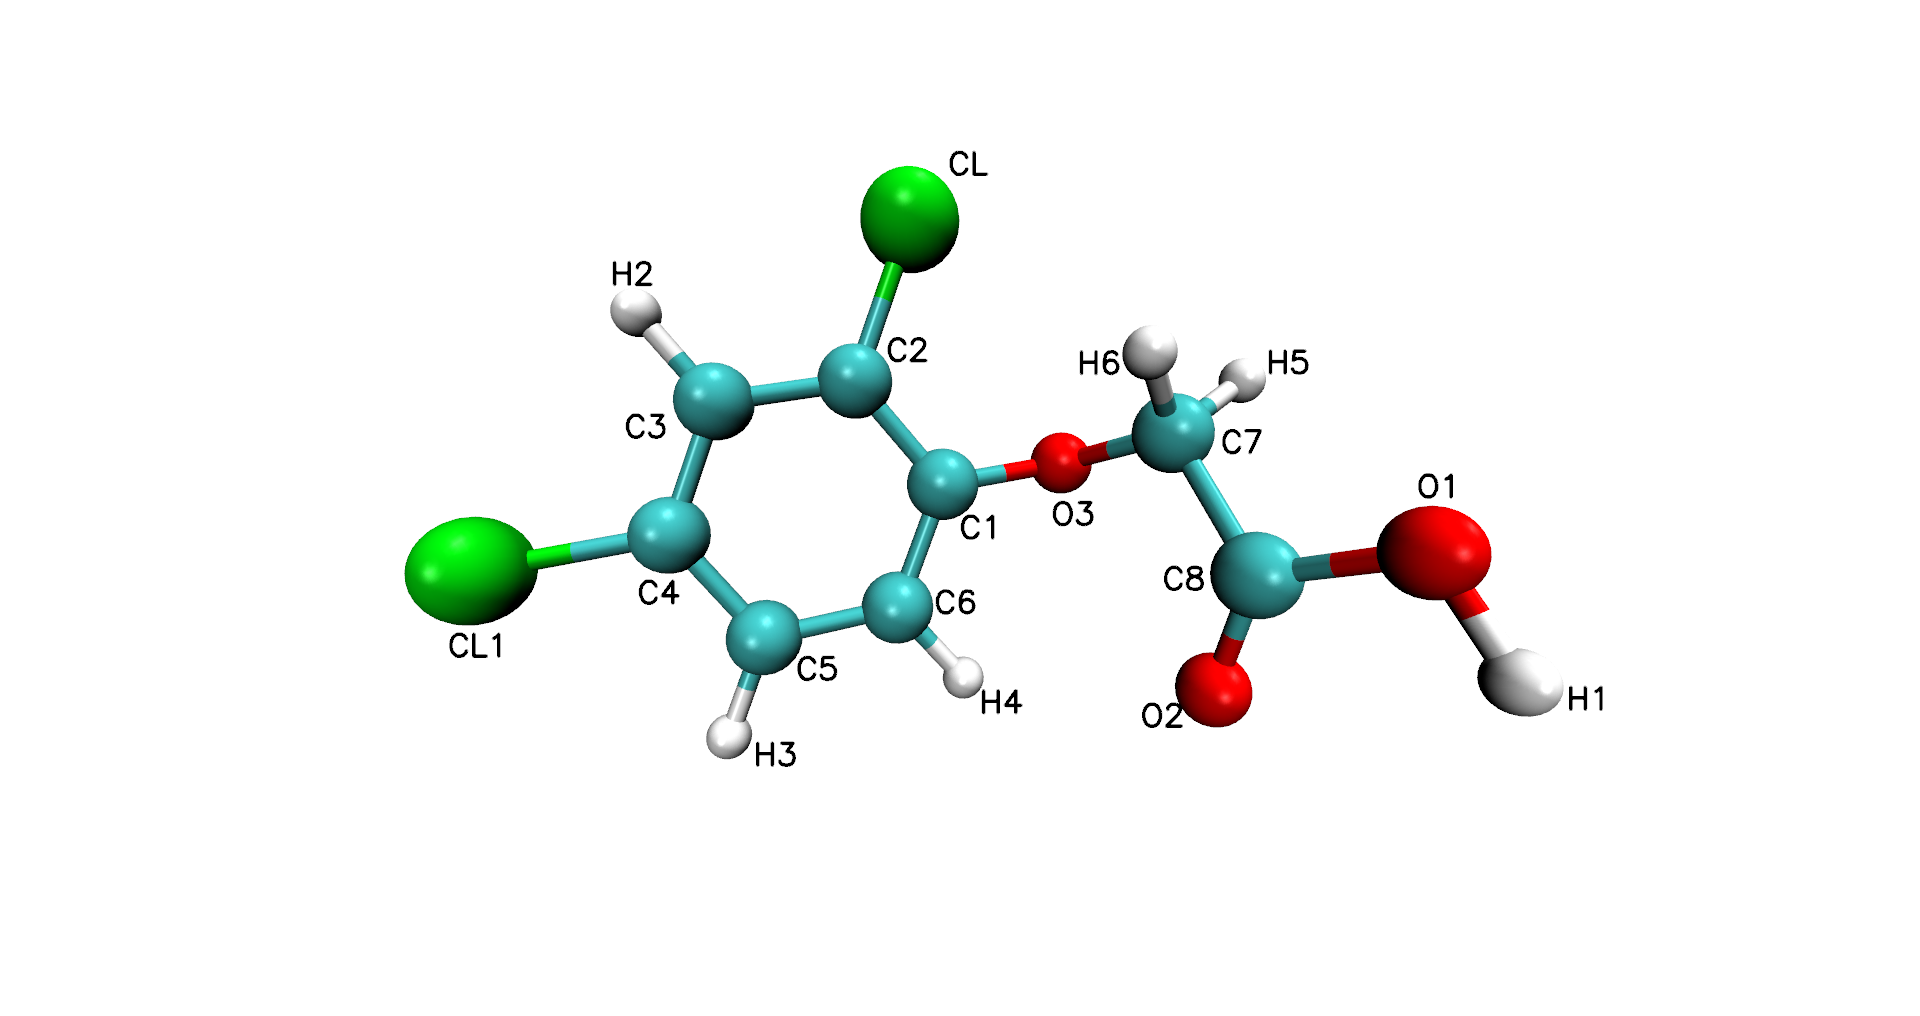
\includegraphics[width=.9\textwidth,keepaspectratio=true]{figura_nueva_tarea.png}
    \caption{Molécula 2,4-D}
    \label{fig:24Dfigure}
\end{figure}

\newpage

% \begin{table}[!h]
% \caption{\label{tab:cnth2oparameters}
% Parámetros del agua rígida y el nanotubo de carbono. \cite{meng2008}}
% \centering
% \begin{tabular}{| c | c || c | c |}
% % &$r_c$ (\AA)&
% % &$r_c$ (\AA)\\
% \hline
% \large{$\epsilon_{cc}$}\footnotemark[1] & 0.4058 kJ/mol & {\large q}_O & -0.8476 e \\
% \large{$\epsilon_{oo}$}\footnotemark[1]& 0.6502 kJ/mol &{\large q}_H& 0.4238 e \\
% \large{$\epsilon_{co}$}\footnotemark[1]& 0.5137 kJ/mol &{\large K}^b_{CC}& 3.2236X10^6 $\frac{kJ}{mol\ nm^4}$\\
% \large{$\sigma_{cc}$}\footnotemark[1]&   3.361         &{\large b}_{ij}& 1.42 \AA\\
% \large{$\sigma_{oo}$}\footnotemark[1]&   3.166         &{\large K}^{$\theta$}_{CCC}& $560 \frac{kJ}{mol}$ \\
% \large{$\sigma_{co}$}\footnotemark[1]&   3.262         &{\large $\theta$}^0_{ijk}& $120^{\circ}$ \\
% {\large r}_{OH}& 1 \AA                                 &{\large k}^{$\phi$}_{CCCC}& 5.86 $\frac{kJ}{mol}$ \\
% {\large $\theta$}_{HOH}& 109.47^{\circ}                &{\large $\phi$}_s& $180^{\circ}$ \\
% \hline
% \end{tabular}
% \footnotetext[1]{Provided in GROMACS}
% \end{table}

% [ moleculetype ]
% ; Name   nrexcl
% SAYK     3
% [ atoms ]
% ;  nr  type  resnr  resid  atom  cgnr  charge    mass
%     1 CLAro    1    SAYK    CL1    1   -0.095  35.4530
%     2  CAro    1    SAYK     C4    2   -0.125  12.0110
%     3  CAro    1    SAYK     C3    3    0.070  12.0110
%     4    HC    1    SAYK     H2    4    0.116   1.0080
%     5  CAro    1    SAYK     C2    5   -0.185  12.0110
%     6 CLAro    1    SAYK     CL    6   -0.070  35.4530
%     7  CAro    1    SAYK     C1    7    0.491  12.0110
%     8  CAro    1    SAYK     C6    8   -0.375  12.0110
%     9    HC    1    SAYK     H4    9    0.212   1.0080
%   10  CAro    1    SAYK     C5   10    0.037  12.0110
%   11    HC    1    SAYK     H3   11    0.130   1.0080
%   12    OE    1    SAYK     O3   12   -0.431  15.9994
%   13  CPos    1    SAYK     C7   13    0.038  12.0110
%   14    HC    1    SAYK     H5   14    0.099   1.0080
%   15    HC    1    SAYK     H6   15    0.099   1.0080
%   16  CPos    1    SAYK     C8   16    0.683  12.0110
%   17 OEOpt    1    SAYK     O2   17   -0.549  15.9994
%   18    OA    1    SAYK     O1   18   -0.610  15.9994
%   19  HS14    1    SAYK     H1   19    0.465   1.0080
% ; total charge of the molecule:   0.000
% [ bonds ]
% ;  ai   aj  funct   c0         c1
%     1    2    2   0.1760   1.4366e+06
%     2    3    2   0.1390   8.6600e+06
%     2   10    2   0.1390   8.6600e+06
%     3    4    2   0.1090   1.2300e+07
%     3    5    2   0.1390   8.6600e+06
%     5    6    2   0.1760   1.4366e+06
%     5    7    2   0.1400   8.5400e+06
%     7    8    2   0.1390   8.6600e+06
%     7   12    2   0.1380   1.1000e+07
%     8    9    2   0.1090   1.2300e+07
%     8   10    2   0.1390   8.6600e+06
%   10   11    2   0.1090   1.2300e+07
%   12   13    2   0.1430   8.1800e+06
%   13   14    2   0.1090   1.2300e+07
%   13   15    2   0.1090   1.2300e+07
%   13   16    2   0.1530   7.1500e+06
%   16   17    2   0.1210   1.2977e+07
%   16   18    2   0.1350   1.0300e+07
%   18   19    2   0.0983   9.8314e+06
% [ pairs ]
% ;  ai   aj  funct  ;  all 1-4 pairs but the ones excluded in GROMOS itp
%     1    4    1
%     1    5    1
%     1    8    1
%     1   11    1
%     2    6    1
%     2    9    1
%     3   11    1
%     3   12    1
%     4    6    1
%     4    7    1
%     4   10    1
%     5    9    1
%     5   13    1
%     6    8    1
%     6   12    1
%     7   11    1
%     7   14    1
%     7   15    1
%     7   16    1
%     8   13    1
%     9   11    1
%     9   12    1
%   10   12    1
%   12   17    1
%   12   18    1
%   13   19    1
%   14   17    1
%   14   18    1
%   15   17    1
%   15   18    1
%   17   19    1
% [ angles ]
% ;  ai   aj   ak  funct   angle     fc
%     1    2    3    2    120.00   560.00
%     1    2   10    2    120.00   560.00
%     3    2   10    2    120.00   560.00
%     2    3    4    2    120.00   505.00
%     2    3    5    2    120.00   560.00
%     4    3    5    2    120.00   505.00
%     3    5    6    2    120.00   560.00
%     3    5    7    2    120.00   560.00
%     6    5    7    2    120.00   560.00
%     5    7    8    2    120.00   560.00
%     5    7   12    2    121.00   685.00
%     8    7   12    2    120.00   560.00
%     7    8    9    2    120.00   505.00
%     7    8   10    2    120.00   560.00
%     9    8   10    2    120.00   505.00
%     2   10    8    2    120.00   560.00
%     2   10   11    2    120.00   505.00
%     8   10   11    2    120.00   505.00
%     7   12   13    2    119.00  2211.40
%   12   13   14    2    106.75   503.00
%   12   13   15    2    106.75   503.00
%   12   13   16    2    111.00   530.00
%   14   13   15    2    107.57   484.00
%   14   13   16    2    109.60   450.00
%   15   13   16    2    109.60   450.00
%   13   16   17    2    126.00   640.00
%   13   16   18    2    109.50   520.00
%   17   16   18    2    124.00   730.00
%   16   18   19    2    109.50   450.00
% [ dihedrals ]
% ; GROMOS improper dihedrals
% ;  ai   aj   ak   al  funct   angle     fc
%     7    5    8   12    2      0.00   167.36
%     5    3    6    7    2      0.00   167.36
%     3    2    4    5    2      0.00   167.36
%     2    1    3   10    2      0.00   167.36
%   10    2    8   11    2      0.00   167.36
%     8    7    9   10    2      0.00   167.36
%   16   13   17   18    2      0.00   167.36
% [ dihedrals ]
% ;  ai   aj   ak   al  funct    ph0      cp     mult
%     2    3    5    7    1    180.00    41.80    2
%     3    2   10    8    1    180.00    41.80    2
%     3    5    7    8    1    180.00    41.80    2
%     5    7    8   10    1    180.00    41.80    2
%     5    7   12   13    1      0.00     0.42    2
%     7    8   10    2    1    180.00    41.80    2
%     7   12   13   16    1      0.00     1.26    3
%   10    2    3    5    1    180.00    41.80    2
%   12   13   16   18    1    180.00     1.00    6
%   17   16   18   19    1    180.00     7.11    2
% [ exclusions ]
% ;  ai   aj  funct  ;  GROMOS 1-4 exclusions
%     2    7
%     3    8
%     5   10

\begin{table}[!h]
    \centering
    \begin{tabular}{|c|c|}
    \hline
    \large{$q_{\text{molécula}}$} & q(e) \\
    \hline
    \large{$q_{CL}$} & -0.070 e \\
    \large{$q_{CL1}$} & -0.095 e \\
    \large{$q_{C1}$} & 0.491 e \\
    \large{$q_{C2}$} & -0.185 e \\
    \large{$q_{C3}$} & 0.070 e \\
    \large{$q_{C4}$} & -0.125 e \\
    \large{$q_{C5}$} & 0.037 e \\
    \large{$q_{C6}$} & -0.375 e \\
    \large{$q_{C7}$} & 0.038 e \\
    \large{$q_{C8}$} & 0.683 e \\
    \large{$q_{H1}$} & 0.465 e \\
    \large{$q_{H2}$} & 0.116 e \\
    \large{$q_{H3}$} & 0.130 e \\
    \large{$q_{H4}$} & 0.212 e \\
    \large{$q_{H5}$} & 0.099 e \\
    \large{$q_{H6}$} & 0.099 e \\
    \large{$q_{O1}$} & -0.610 e \\
    \large{$q_{O2}$} & -0.549 e \\
    \large{$q_{O3}$} & -0.431 e \\
    \hline
    \end{tabular}
    \caption{Tabla de cargas en 2,4-D}
    \label{tab:cargas24D}
\end{table}


\begin{table}[!h]
    \centering
    \begin{tabular}{|c|c|}
    \hline
    $K^b_{ij}$ $b_{ij}$   & ($\frac{kJ}{molnm^4}$) (\AA)\\
    % \multicolumn{2}{|c|}{$K^b_{ij}$ ($\frac{kJ}{molnm^4}$) $b_{ij}$ (\AA)}\\
    \hline
    $K^b_{C1-C2}\ b_{C1-C2}$   & 8.5400X$10^6$ 1.400\\
    $K^b_{C2-C3}\ b_{C2-C3}$   & 8.6600X$10^6$ 1.390\\
    $K^b_{C3-C4}\ b_{C3-C4}$   & 8.6600X$10^6$ 1.390\\
    $K^b_{C4-C5}\ b_{C4-C5}$   & 8.6600X$10^6$ 1.390\\
    $K^b_{C5-C6}\ b_{C5-C6}$   & 8.6600X$10^6$ 1.390\\
    $K^b_{C7-C8}\ b_{C7-C8}$   & 7.1500X$10^6$ 1.530\\
    $K^b_{C1-C6}\ b_{C1-C6}$   & 8.6600X$10^6$ 1.390\\
    $K^b_{CL1-C4}\ b_{CL1-C4}$ & 1.4366X$10^6$ 1.760\\
    $K^b_{C2-CL}\ b_{C2-CL}$   & 1.4366X$10^6$ 1.760\\
    $K^b_{C5-H3}\ b_{C5-H3}$   & 1.2300X$10^7$ 1.090\\
    $K^b_{C6-H4}\ b_{C6-H4}$   & 1.2300X$10^7$ 1.090\\
    $K^b_{C3-H2}\ b_{C3-H2}$   & 1.2300X$10^7$ 1.090\\
    $K^b_{C1-O3}\ b_{C1-O3}$   & 1.1000X$10^7$ 1.380\\
    $K^b_{O3-C7}\ b_{O3-C7}$   & 8.1800X$10^6$ 1.430\\
    $K^b_{H5-C7}\ b_{H5-C7}$   & 1.2300X$10^7$ 1.090\\
    $K^b_{H6-C7}\ b_{H6-C7}$   & 1.2300X$10^7$ 1.090\\
    $K^b_{O2-C8}\ b_{O2-C8}$   & 1.2977X$10^7$ 1.210\\
    $K^b_{O-C8} \ b_{O1-C8}$   & 1.0300X$10^7$ 1.210\\
    $K^b_{O1-H1}\ b_{O1-H1}$   & 9.8314X$10^6$ 0.983\\
    \hline
    \end{tabular}
    \caption{Tabla de parámetros del potencial de enlace de 2,4-D}
    \label{tab:enlace24D}
\end{table}



\begin{table}[!h]
    \centering
    \begin{tabular}{|c|c|}
    \hline
    $K^{\theta}_{ijk}$ $\theta^0_{ijk}$& $\frac{kJ}{mol}$\quad $^{\circ}$\\
    \hline
    $K^{\theta}_{C3-C4-CL1} \theta^0_{C3-C4-CL1}$& 560 120\\
    $K^{\theta}_{C4-C5-CL1} \theta^0_{C4-C5-CL1}$& 560 120\\
    $K^{\theta}_{C3-C4-C5} \theta^0_{C3-C4-C5}$& 560 120\\
    $K^{\theta}_{C2-C3-C4} \theta^0_{C2-C3-C4}$& 560 120\\
    $K^{\theta}_{C2-C3-CL} \theta^0_{C2-C3-CL}$& 560 120\\
    $K^{\theta}_{C1-C2-C3} \theta^0_{C1-C2-C3}$& 560 120\\
    $K^{\theta}_{C1-C2-CL} \theta^0_{C1-C2-CL}$& 560 120\\
    $K^{\theta}_{C1-C2-C6} \theta^0_{C1-C2-C6}$& 560 120\\
    $K^{\theta}_{C1-C6-O3} \theta^0_{C1-C6-O3}$& 560 120\\
    $K^{\theta}_{C1-C6-C5} \theta^0_{C1-C6-C5}$& 560 120\\
    $K^{\theta}_{C4-C5-C6} \theta^0_{C4-C5-C6}$& 560 120\\

    $K^{\theta}_{C3-C4-H2} \theta^0_{C3-C4-H2}$& 505 120\\
    $K^{\theta}_{C2-C3-H2} \theta^0_{C2-C3-H2}$& 505 120\\
    $K^{\theta}_{C1-C6-H4} \theta^0_{C1-C6-H4}$& 505 120\\
    $K^{\theta}_{C5-C6-H4} \theta^0_{C5-C6-H4}$& 505 120\\
    $K^{\theta}_{C4-C5-H3} \theta^0_{C4-C5-H3}$& 505 120\\
    $K^{\theta}_{C5-C6-H3} \theta^0_{C5-C6-H3}$& 505 120\\
    
    $K^{\theta}_{C7-C8-H5} \theta^0_{C7-C8-H5}$& 450 109.60\\
    $K^{\theta}_{C7-C8-H6} \theta^0_{C7-C8-H6}$& 450 109.60\\
    $K^{\theta}_{C8-O1-H1} \theta^0_{C8-O1-H1}$& 450 109.50\\
    $K^{\theta}_{C7-C8-O1} \theta^0_{C7-C8-O1}$& 520 109.50\\
    
    $K^{\theta}_{C7-H5-H6} \theta^0_{C7-H5-H6}$& 484 107.57\\
    $K^{\theta}_{O3-C7-H5} \theta^0_{O3-C7-H5}$& 503 106.75\\
    $K^{\theta}_{O3-C7-H6} \theta^0_{O3-C7-H6}$& 503 106.75\\
    $K^{\theta}_{O3-C7-C8} \theta^0_{O3-C7-C8}$& 530 111\\
    $K^{\theta}_{C7-C8-O2} \theta^0_{C7-C8-O2}$& 640 126\\
    $K^{\theta}_{C1-C2-O3} \theta^0_{C1-C2-O3}$& 685 121\\
    $K^{\theta}_{C8-O2-O1} \theta^0_{C8-O2-O1}$& 730 124\\
    $K^{\theta}_{C1-C7-O3} \theta^0_{C1-C7-O3}$& 2211.40 119\\
    \hline
    \end{tabular}
    \caption{Tabla de parametros de ángulos de 2,4-D}
    \label{tab:angulos24D}
\end{table}

\begin{table}[!h]
    \centering
    \begin{tabular}{|c|c|}
    \hline
    $k^{\xi}_{ijkl}$ $\xi^{0}_{ijkl}$ & $\frac{kJ}{molrad^2}$\quad $^{\circ}$ \\
    \hline
    $k^{\xi}_{C1-C2-C6-O3}$ $\xi_{0}$ & 167.36 0\\
    $k^{\xi}_{C1-C2-C3-CL}$ $\xi_{0}$ & 167.36 0\\
    $k^{\xi}_{C2-C3-C4-H2}$ $\xi_{0}$ & 167.36 0\\
    $k^{\xi}_{C3-C4-C5-CL1}$ $\xi_{0}$ & 167.36 0 \\
    $k^{\xi}_{C4-C5-C6-H3}$ $\xi_{0}$ & 167.36 0\\
    $k^{\xi}_{C1-C5-C6-H4}$ $\xi_{0}$ & 167.36 0\\
    $k^{\xi}_{C7-C8-O1-O2}$ $\xi_{0}$ & 167.36 0\\
    \hline
    $k^{\phi}_{ijkl}$ $\phi^s_{ijkl}$ & $\frac{kJ}{mol}$\quad $^{\circ}$\\
    \hline
    $k^{\phi}_{C1-C2-C3-C4}$ $\phi_s$ & 41.80 180\\
    $k^{\phi}_{C3-C4-C5-C6}$ $\phi_s$ & 41.80 180\\
    $k^{\phi}_{C1-C2-C3-C6}$ $\phi_s$ & 41.80 180\\
    $k^{\phi}_{C1-C2-C5-C6}$ $\phi_s$ & 41.80 180\\
    $k^{\phi}_{C1-C4-C5-C6}$ $\phi_s$ & 41.80 180\\
    $k^{\phi}_{C2-C3-C4-C5}$ $\phi_s$ & 41.80 180\\
    $k^{\phi}_{C7-C8-O1-O3}$ $\phi_s$ n & 1.00 180 6\\
    $k^{\phi}_{C8-O1-O2-H1}$ $\phi_s$ n & 7.11 180 2\\
    $k^{\phi}_{C1-C2-O3-C7}$ $\phi_s$ n & 0.42 0 2\\
    $k^{\phi}_{C1-C7-C8-O3}$ $\phi_s$ n & 1.26 0 3\\
    \hline
    \end{tabular}
    \caption{Tabla de parámetros del potencial de ángulos diedros de 2,4-D}
    \label{tab:angulosdih24D}
\end{table}

\newpage
%               c6              c12                sigma                 epsilon
% C    CLAro      1  0.003974417     6.381584e-06       0.3421967204782815    0.6188115086273643
% C     CAro      1  0.002340624     4.690642e-06      sigma: 0.3550722828524636, epsilon: 0.29199205084165447
% HC	C	      1	4.450960E-04	2.733060E-07      sigma: 0.2915407359639445, epsilon: 0.18121670327032705
% C	OE	          1	2.300953E-03	2.444200E-06          sigma: 0.31942690878969837, epsilon: 0.541525315871144
% C     CPos      1  0.0021771       2.222e-06         sigma: 0.31730550936068447, epsilon: 0.5332768238073807
% C    OEOpt      1  0.00268896      4.85507e-06       sigma: 0.34895427699812803, epsilon: 0.37231728284041216
% C     HS14      1  0               0           
% C	OA	          1	2.300953E-03	2.444200E-06          sigma: 0.31942690878969837, epsilon: 0.541525315871144

% OA    CLAro     1  0.003907054     3.1592e-06       sigma: 0.3052258307853132, epsilon: 1.2079854835809698
% OW    CLAro     1  0.004202794     4.661256e-06     sigma: 0.3217319135230157, epsilon: 0.9473561099431141
% HS14    CLAro   1  0               0
% CLAro    OEOpt  1  0.004565897     6.27532e-06   sigma: 0.33344045848470744, epsilon: 0.830531965485784
% CLAro     CAro  1  0.003974417     6.062792e-06  sigma: 0.3392864686204393, epsilon: 0.6513496789057335
% CLAro     CPos  1  0.00369675      2.872e-06     sigma: 0.3031987401164613, epsilon: 1.1895857035602366
% OE    CLAro     1  0.003907054     3.231e-06        sigma: 0.30637119042109173, epsilon: 1.181141361723615
% HC    CLAro     1  0.00075578      3.53256e-07      sigma: 0.27857941708920847, epsilon: 0.4042418305704644

% OE     CAro     1  0.002300953     2.3221e-06       sigma: 0.3167103054468882, epsilon: 0.5699996456019336
% OA     CAro     1  0.002300953     2.3221e-06       sigma: 0.3167103054468882, epsilon: 0.5699996456019336
% OW     CAro     1  0.002475121     3.426153e-06     sigma: 0.33383744896554585, epsilon: 0.44701914688580746
% HC     CAro     1  0.000445096     2.59653e-07      sigma: 0.2890612938252534, epsilon: 0.19074538828359391
% HS14     CAro   1  0               0
% OEOpt     CAro  1  0.00268896      4.612535e-06  sigma: 0.34598655471395084, epsilon: 0.39189436403192596
% CAro     CPos   1  0.0021771       2.111e-06      sigma: 0.3146069477063536, epsilon: 0.56131743368072
% CAro     CAro   1  0.002340624     4.456321e-06   sigma: 0.3520525292750613, epsilon: 0.30734549359078933

% HC	OA	      1	4.375520E-04	1.353000E-07      sigma: 0.2600427123263571, epsilon: 0.3537541624242424
% HC	OE	      1	4.375520E-04	1.353000E-07      sigma: 0.2600427123263571, epsilon: 0.3537541624242424
% HC	OW	      1	4.706720E-04	1.996290E-07      sigma: 0.2741053705029336, epsilon: 0.2774297967529768
% HC     HS14     1  8.464e-05       1.5129e-08       sigma: 0.23734081428097492, epsilon: 0.1183807521977659
% HC    OEOpt     1  0.000511336     2.68755e-07      sigma: 0.28408067888820254, epsilon: 0.24321827026101842
% HC     CPos     1  0.000414        1.23e-07         sigma: 0.2583156954670584, epsilon: 0.34836585365853656
    
% OE     HS14     1  0               0     
% OE    OEOpt     1  0.002643385     2.4035e-06       sigma: 0.31125329012564956, epsilon: 0.7268030224906386
% OE     CPos     1  0.0021402       1.1e-06          sigma: 0.28302386291723314, epsilon: 1.0410127363636363
    
% OA     CPos     1  0.0021402       1.1e-06          sigma: 0.28302386291723314, epsilon: 1.0410127363636363
% OW     CPos     1  0.0023022       1.623e-06        sigma: 0.2983293017984591, epsilon: 0.8164086321626617
% HS14     CPos   1  0               0
% OEOpt     CPos  1  0.0025011       2.185e-06     sigma: 0.3091861733013462, epsilon: 0.7157324038901602

% OA    OEOpt     1  0.002643385     2.4035e-06       sigma: 0.31125329012564956, epsilon: 0.7268030224906386
% OW    OEOpt     1  0.002843473     3.546255e-06     sigma: 0.32808532768562954, epsilon: 0.5699913501517093
% HS14    OEOpt   1  0               0

% OA     HS14     1  0               0

% OW     HS14     1  0               0
% HS14     HS14   1  8.464e-05       1.5129e-08     sigma: 0.23734081428097492, epsilon: 0.1183807521977659

La tabla \ref{tab:lennardjonesall} muestran los parámetros Lennard-Jones para 2,4-D con el nanotubo del carbono, con agua y consigo misma. La lista \ref{tab:24Ditp} es el tipo de átomo dentro de GROMACS para cada átomo de 2,4-D en la figura \ref{fig:24Dfigure} descrito en el archivo itp.

\begin{table}[!h]
    \centering
    \begin{tabular}{|c|c|}
    \hline
    tipo & átomo\\
    \hline
   CLAro & CL1\\
    CAro &  C4\\
    CAro &  C3\\
      HC &  H2\\
    CAro &  C2\\
   CLAro &  CL\\
    CAro &  C1\\
    CAro &  C6\\
      HC &  H4\\
    CAro &  C5\\
      HC &  H3\\
      OE &  O3\\
    CPos &  C7\\
      HC &  H5\\
      HC &  H6\\
    CPos &  C8\\
   OEOpt &  O2\\
      OA &  O1\\
    HS14 &  H1\\
    \hline
    \end{tabular}
    \caption{Lista de átomos en el archivo .itp de 2,4-D}
    \label{tab:24Ditp}
\end{table}


\begin{table}[!h]
    \centering
    \begin{tabular}{|c|c|}
    \hline
        $a_1$ $a_2$ & $\sigma$(nm) $\epsilon$(kJ/mol) \\
        \hline
        C    CLAro      &     0.3421967204782815 0.6188115086273643\\
        C     CAro      &     0.3550722828524636 0.29199205084165447\\
        HC	C	        &     0.2915407359639445 0.18121670327032705\\
        C	OE	        &     0.31942690878969837 0.541525315871144\\
        C     CPos      &     0.31730550936068447 0.5332768238073807\\
        C    OEOpt      &     0.34895427699812803 0.37231728284041216\\
        C     HS14      &     0                   0\\
        C	OA	        &     0.31942690878969837 0.541525315871144\\
        OA    CLAro     &     0.3052258307853132 1.2079854835809698\\
        OW    CLAro     &     0.3217319135230157 0.9473561099431141\\
        HS14    CLAro   &     0                   0\\
        CLAro    OEOpt  &     0.33344045848470744 0.830531965485784\\
        CLAro     CAro  &     0.3392864686204393 0.6513496789057335\\
        CLAro     CPos  &     0.3031987401164613 1.1895857035602366\\
        OE    CLAro     &     0.30637119042109173 1.181141361723615\\
        HC    CLAro     &     0.27857941708920847 0.4042418305704644\\
        OE     CAro     &     0.3167103054468882 0.5699996456019336\\
        OA     CAro     &     0.3167103054468882 0.5699996456019336\\
        OW     CAro     &     0.33383744896554585 0.44701914688580746\\
        HC     CAro     &     0.2890612938252534 0.19074538828359391\\
        HS14     CAro   &     0                   0\\
        OEOpt     CAro  &     0.34598655471395084 0.39189436403192596\\
        CAro     CPos   &     0.3146069477063536 0.56131743368072\\
        CAro     CAro   &     0.3520525292750613 0.30734549359078933\\
        HC	OW	        &     0.2741053705029336 0.2774297967529768\\
        HC	OE	        &     0.2600427123263571 0.3537541624242424\\
        HC	OA	        &     0.2600427123263571 0.3537541624242424\\
        HC     HS14     &     0.23734081428097492 0.1183807521977659\\
        HC    OEOpt     &     0.28408067888820254 0.24321827026101842\\
        HC     CPos     &     0.2583156954670584 0.34836585365853656\\
        OE     HS14     &     0                   0\\
        OE    OEOpt     &     0.31125329012564956 0.7268030224906386\\
        OE     CPos     &     0.28302386291723314 1.0410127363636363\\
        OA     CPos     &     0.28302386291723314 1.0410127363636363\\
        OW     CPos     &     0.2983293017984591 0.8164086321626617\\
        HS14     CPos   &     0                   0\\
        OEOpt     CPos  &     0.3091861733013462 0.7157324038901602\\
        OA    OEOpt     &     0.31125329012564956 0.7268030224906386\\
        OW    OEOpt     &     0.32808532768562954 0.5699913501517093\\
        HS14    OEOpt   &     0                   0\\
        OA     HS14     &     0                   0\\
        OW     HS14     &     0                   0\\
        HS14     HS14   &     0.23734081428097492 0.1183807521977659\\
        \hline
    \end{tabular}
    \caption{Tabla de parámetros del potencial de Lennard-Jones de 2,4-D}
    \label{tab:lennardjonesall}
\end{table}
